\documentclass[aspectratio=169]{beamer}

\usepackage[T1]{fontenc}
\usepackage{lmodern}
\usepackage{tikz}
\usetikzlibrary{arrows.meta,positioning,calc,fit}

\setbeamertemplate{navigation symbols}{}
\setbeamercolor{background canvas}{bg=white}

\definecolor{ink}{RGB}{55,55,55}
\definecolor{soft}{RGB}{110,110,110}

\begin{document}

\begin{frame}[plain]
\centering
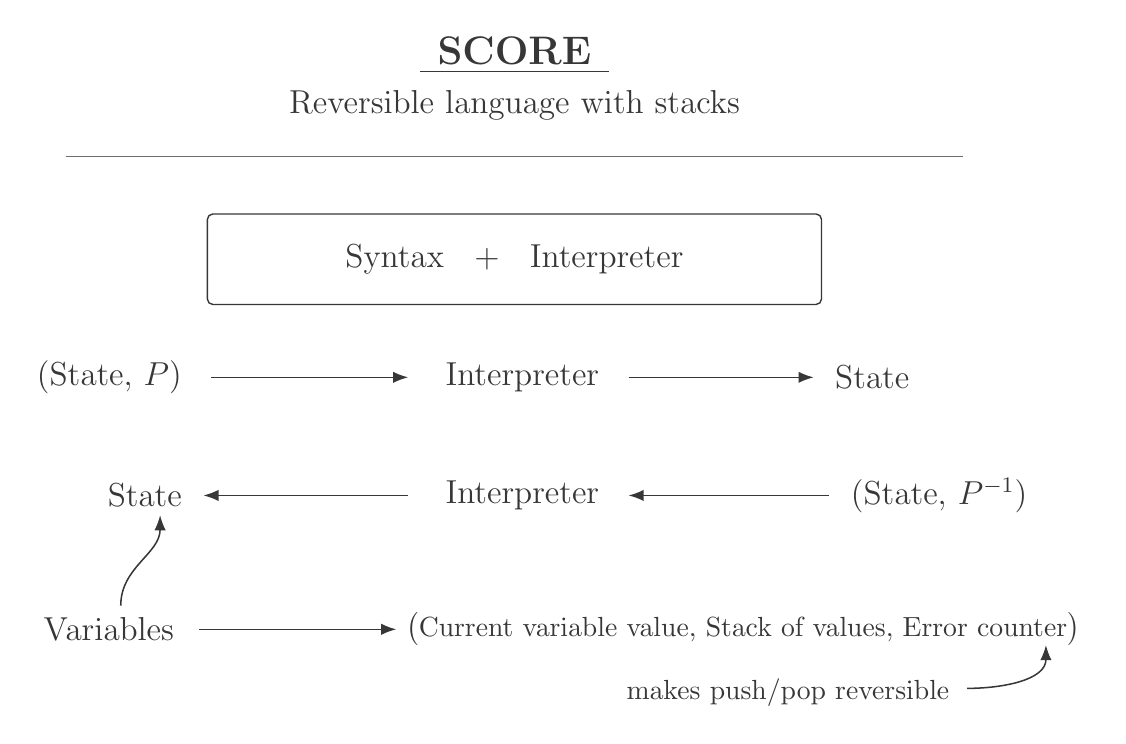
\begin{tikzpicture}[
    x=1cm,y=1cm,
    >=Latex,
    text=ink,
    every node/.style={font=\large},
    box/.style={
        draw=ink,
        rounded corners=2pt,
        line width=0.5pt,
        minimum height=1.15cm,
        inner sep=6pt,
        align=center
    },
    lbl/.style={font=\large, text=ink},
    smalllbl/.style={font=\normalsize, text=ink},
    arr/.style={->, line width=0.55pt, draw=ink},
    rev/.style={<-, line width=0.55pt, draw=ink}
]

% Title
\node[font=\Large\bfseries] (title) at (0,4.9) {SCORE};
\draw[ink, line width=0.45pt] (-1.2,4.63) -- (1.2,4.63);
\node[font=\large] at (0,4.2) {Reversible language with stacks};

% Separator line
\draw[soft, line width=0.35pt] (-5.7,3.55) -- (5.7,3.55);

% Syntax + Interpreter box
\node[box, minimum width=7.8cm] (syntax) at (0,2.25) {Syntax \hspace{0.6em}+\hspace{0.6em} Interpreter};

% Forward interpretation
\node[lbl, anchor=east] (sp) at (-4.1,0.75) {$(\mathrm{State},\,P)$};
\node[lbl] (interp1) at (0.1,0.75) {Interpreter};
\node[lbl, anchor=west] (state1) at (3.95,0.75) {$\mathrm{State}$};
\draw[arr] ($(sp.east)+(0.25,0)$) -- ($(interp1.west)+(-0.35,0)$);
\draw[arr] ($(interp1.east)+(0.25,0)$) -- ($(state1.west)+(-0.15,0)$);

% Reverse interpretation
\node[lbl, anchor=east] (state2) at (-4.1,-0.75) {$\mathrm{State}$};
\node[lbl] (interp2) at (0.1,-0.75) {Interpreter};
\node[lbl, anchor=west] (pinv) at (4.15,-0.75) {$(\mathrm{State},\,P^{-1})$};
\draw[rev] ($(state2.east)+(0.15,0)$) -- ($(interp2.west)+(-0.35,0)$);
\draw[rev] ($(interp2.east)+(0.25,0)$) -- ($(pinv.west)+(-0.15,0)$);

%% Variables to state
%\node[lbl, anchor=east] (vars) at (-2.2,-2.45) {Variables};
%\node[smalllbl, align=left, anchor=west] (tuple) at (.5,-2.45)
%{
%$\bigl($Current variable value, Stack of values, Error counter$\bigr)$
%};

% Variables to state
\node[lbl, anchor=east] (vars) at (-4.2,-2.45) {Variables};
\node[smalllbl, align=left, anchor=west] (tuple) at (-1.5,-2.45)
{
$\bigl($Current variable value, Stack of values, Error counter$\bigr)$
};

% Arrow from Variables to tuple (centered on target node)
\draw[arr] ($(vars.east)+(0.2,0)$) -- (tuple.west);

% Curved arrow from Variables notion up to State
\draw[arr] (-5,-2.15) to[out=90,in=-90] (-4.5,-1.0);

% Bottom note (named node)
\node[smalllbl, anchor=west] (note) at (1.3,-3.25) {makes push/pop reversible};

% Coordinate near "Error counter" (right side of tuple)
\coordinate (err) at ($(tuple.east)+(-0.3,0)$);

% Arrow from note to "Error counter"
%\draw[arr] (note.north west) to[out=0,in=-60] (err);
\draw[arr] (5.75,-3.20) to[out=0,in=-90] (6.75,-2.65);

\end{tikzpicture}
\end{frame}

\end{document}




%\documentclass[aspectratio=169]{beamer}
%
%\usepackage[T1]{fontenc}
%\usepackage{lmodern}
%\usepackage{tikz}
%\usetikzlibrary{arrows.meta,positioning,calc,fit}
%
%\setbeamertemplate{navigation symbols}{}
%\setbeamercolor{background canvas}{bg=white}
%
%\definecolor{ink}{RGB}{55,55,55}
%\definecolor{soft}{RGB}{110,110,110}
%
%\begin{document}
%
%\begin{frame}[plain]
%\centering
%\begin{tikzpicture}[
%    x=1cm,y=1cm,
%    >=Latex,
%    text=ink,
%    every node/.style={font=\large},
%    box/.style={
%        draw=ink,
%        rounded corners=2pt,
%        line width=0.5pt,
%        minimum height=1.15cm,
%        inner sep=6pt,
%        align=center
%    },
%    lbl/.style={font=\large, text=ink},
%    smalllbl/.style={font=\normalsize, text=ink},
%    arr/.style={->, line width=0.55pt, draw=ink},
%    rev/.style={<-, line width=0.55pt, draw=ink}
%]
%
%% Title
%\node[font=\Large\bfseries] (title) at (0,4.9) {SCORE};
%\draw[ink, line width=0.45pt] (-1.2,4.63) -- (1.2,4.63);
%\node[font=\large] at (0,4.2) {Reversible language with stacks};
%
%% Separator line
%\draw[soft, line width=0.35pt] (-5.7,3.55) -- (5.7,3.55);
%
%% Syntax + Interpreter box
%\node[box, minimum width=7.8cm] (syntax) at (0,2.25) {Syntax \hspace{0.6em}+\hspace{0.6em} Interpreter};
%
%% Forward interpretation
%\node[lbl, anchor=east] (sp) at (-4.1,0.25) {$(\mathrm{State},\,P)$};
%\node[lbl] (interp1) at (0.1,0.25) {Interpreter};
%\node[lbl, anchor=west] (state1) at (3.95,0.25) {$\mathrm{State}$};
%\draw[arr] ($(sp.east)+(0.25,0)$) -- ($(interp1.west)+(-0.35,0)$);
%\draw[arr] ($(interp1.east)+(0.25,0)$) -- ($(state1.west)+(-0.15,0)$);
%
%% Reverse interpretation
%\node[lbl, anchor=east] (state2) at (-4.1,-1.25) {$\mathrm{State}$};
%\node[lbl] (interp2) at (0.1,-1.25) {Interpreter};
%\node[lbl, anchor=west] (pinv) at (4.15,-1.25) {$(\mathrm{State},\,P^{-1})$};
%\draw[rev] ($(state2.east)+(0.15,0)$) -- ($(interp2.west)+(-0.35,0)$);
%\draw[rev] ($(interp2.east)+(0.25,0)$) -- ($(pinv.west)+(-0.15,0)$);
%
%% Variables to state
%\node[lbl, anchor=east] (vars) at (-2.2,-2.95) {Variables};
%\node[smalllbl, align=left, anchor=west] (tuple) at (.5,-2.95)
%{
%$\bigl($Current variable value, Stack of values, Error counter$\bigr)$
%};
%
%\draw[arr] ($(vars.east)+(0.2,0)$) -- ($(tuple.west)+(-0.2,0)$);
%
%% Curved arrow from Variables notion up to State
%\draw[arr] (-3.7,-2.65) to[out=135,in=-120] (-4.0,-1.5);
%
%% Bottom note
%\draw[ink, line width=0.45pt] (0.95,-3.72) -- (5.5,-3.72);
%\node[smalllbl, anchor=west] at (1.3,-4.08) {makes push/pop reversible};
%
%\end{tikzpicture}
%\end{frame}
%
%\end{document}